\begin{figure}[H]
	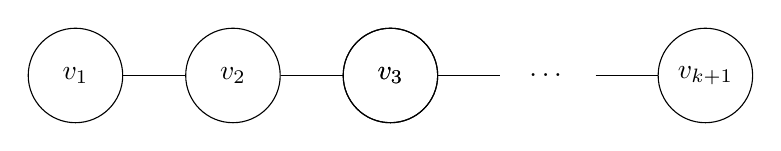
\begin{tikzpicture}[node distance={20mm}, main/.style = {draw, circle}, minimum size=1.2cm]
		\node[main] (1) {$v_1$};
		\node[main] (2) [right of=1] {$v_2$};
		\node[main] (3) [right of=2] {$v_3$};
		\node[main] (3) [right of=2] {$v_3$};
		\node (4) [right of =3] {\dots};
		
		\node[main] (5) [right of=4] {$v_{k + 1}$};
		\draw (1) -- (2);
		\draw (2) -- (3);
		\draw (3) -- (4);
		\draw (4) -- (5);
	\end{tikzpicture}
	\centering
	\caption{Structure $\mathfrak{B}$, consisting of a line of length $k$.}
\end{figure}